\anonsection{Практическая часть}
В этом разделе будут выбраны средства разработки ПО, приведены листинги кода и демонстрация работы программы.

\subsection*{Выбор средств разработки ПО}
В качестве языка программирования выбран Golang. 
Это обусловлено тем, что автор имеет опыт разработки на данном языке, а также наличием пакетов, позволяющих настраивать построение графиков, требуемых для работы.

\subsection*{Листинги кода}
Абстрактное понятие распределение представлено интерфейсом Distribution. Структуры, его реализовывающие, должны иметь четыре функции: для подсчёта плотности случайной величины и функции распределения в конкретной точке, а также на определённом интервале.

На листинге \ref{distLabel} представлен интерфейс Distribution:
\FloatBarrier
\begin{lstinputlisting}[language=go, caption=Интерфейс для реализаций распределений, linerange={1-9}, 
	basicstyle=\footnotesize\ttfamily, frame=single, breaklines=true]{../src/pkg/distribution/distribution.go}
	\label{distLabel}
\end{lstinputlisting}
\FloatBarrier

\newpage

Реализация требуемых распределений в конкретной точке для равномерного распределения представлена на листинге 2:
\FloatBarrier
\begin{lstinputlisting}[language=go, caption=Расчёт значений функций для равномерного распределения, linerange={18-37}, 
	basicstyle=\footnotesize\ttfamily, frame=single, breaklines=true]{../src/pkg/distribution/uniform.go}
	\label{unif}
\end{lstinputlisting}
\FloatBarrier

Реализация поиска плотности в конкретной точке для распределения Эрланга представлена на листинге 3:
\FloatBarrier
\begin{lstinputlisting}[language=go, caption=Расчёт функции плотности для распределения Эрланга, linerange={29-38}, 
	basicstyle=\footnotesize\ttfamily, frame=single, breaklines=true]{../src/pkg/distribution/erlang.go}
	\label{er}
\end{lstinputlisting}
\FloatBarrier

Реализация поиска функции распределения в конкретной точке для распределения Эрланга представлена на листинге 4:
\FloatBarrier
\begin{lstinputlisting}[language=go, caption=Расчёт функции распределения случайной величины для распределения Эрланга, linerange={40-48}, 
	basicstyle=\footnotesize\ttfamily, frame=single, breaklines=true]{../src/pkg/distribution/erlang.go}
	\label{er1}
\end{lstinputlisting}
\FloatBarrier

\subsection*{Демонстрация работы программы}
На рисунке 1 представлен график функции плотности равномерного распределения с заданными параметрами.

\FloatBarrier
\begin{figure}[h]
	\begin{center}
		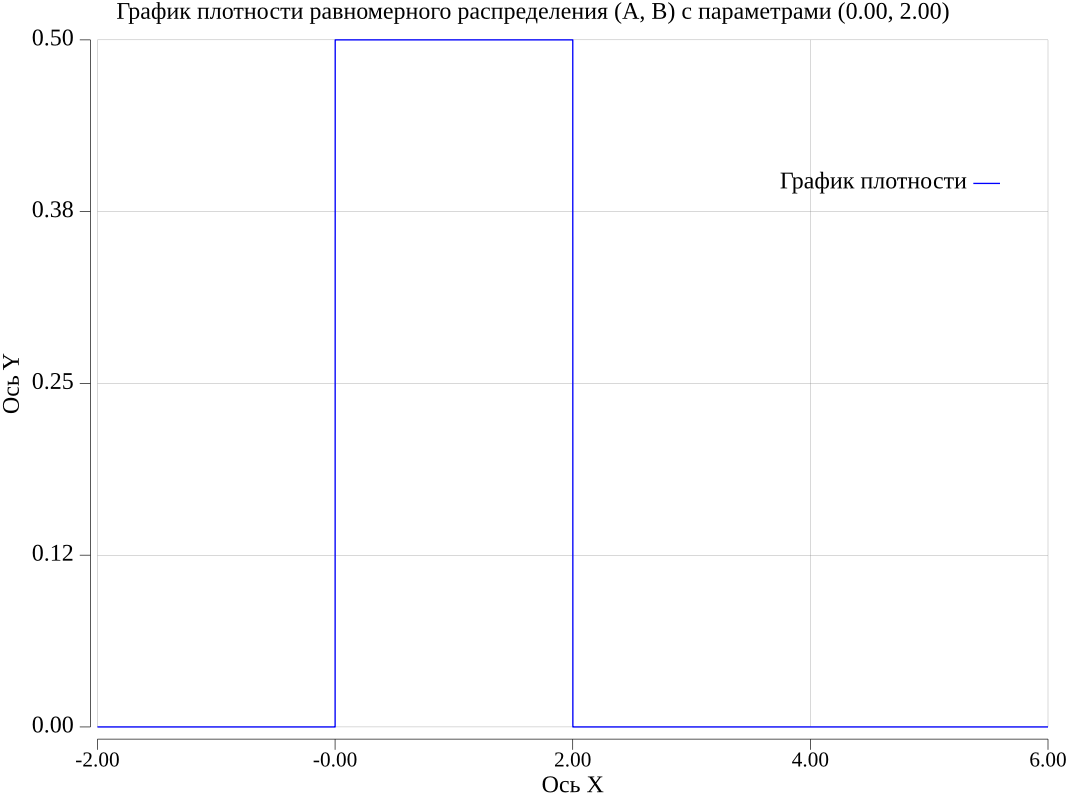
\includegraphics[width=\linewidth, height=11cm]{inc/verProb.png}
	\end{center}
	\caption{Демонстрация построения графика плотности для равномерного распределения}
\end{figure}
\FloatBarrier

На рисунке 2 представлен график функции плотности распределения Эрланга с заданными параметрами.
\FloatBarrier
\begin{figure}[h]
	\begin{center}
		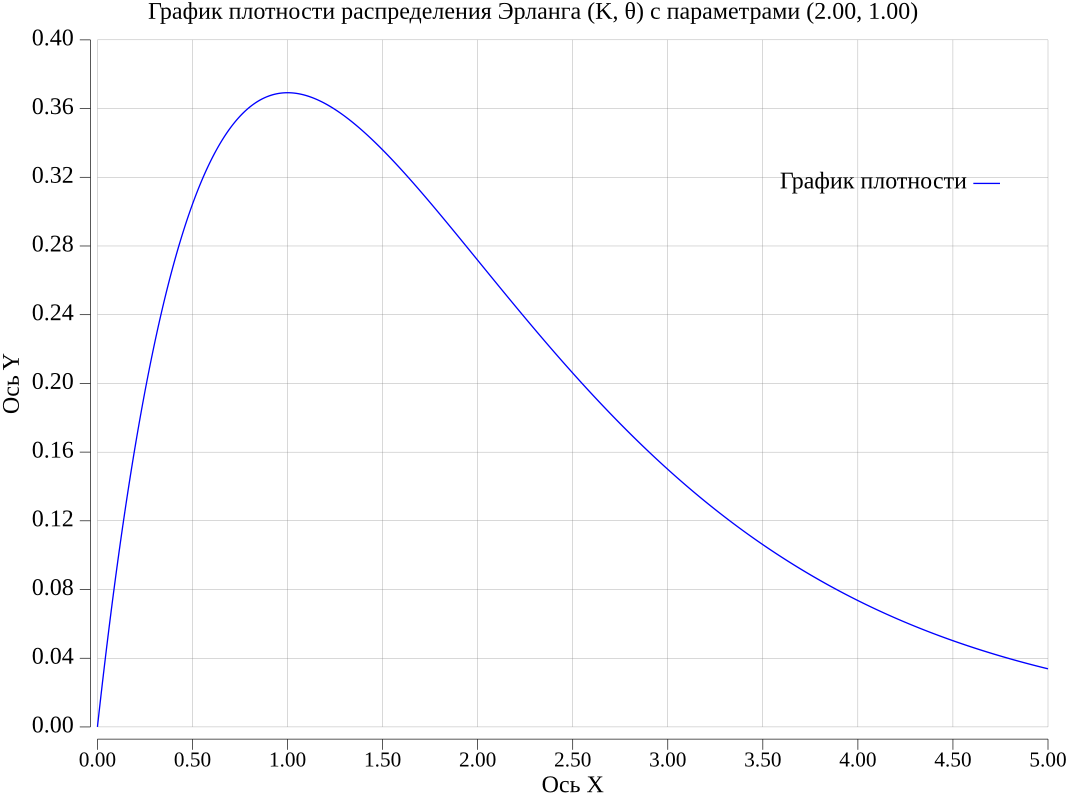
\includegraphics[width=\linewidth]{inc/erlangProb.png}
	\end{center}
	\caption{Демонстрация построения графика плотности для распределения Эрланга}
\end{figure}
\FloatBarrier

\newpage
На рисунке 3 представлен график функции распределения для равномерного распределения с заданными параметрами.
\FloatBarrier
\begin{figure}[h]
	\begin{center}
		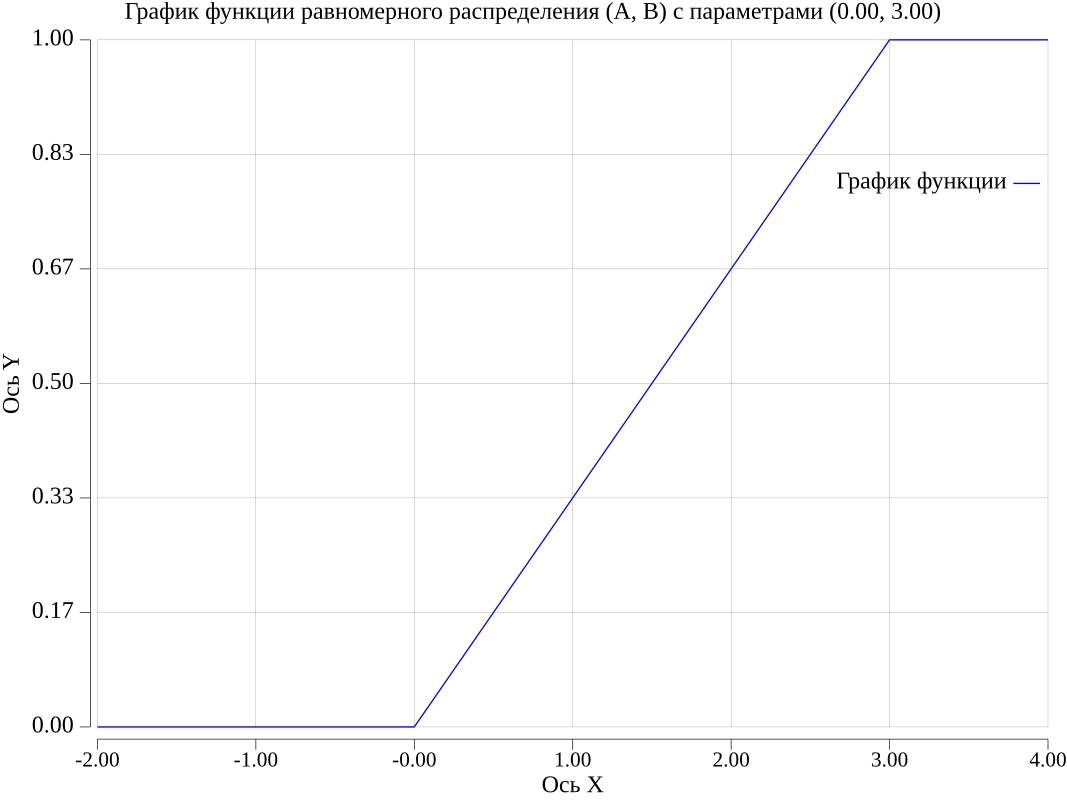
\includegraphics[width=\linewidth]{inc/verFunc.png}
	\end{center}
	\caption{Демонстрация построения графика функции распределения для равномерного распределения}
\end{figure}
\FloatBarrier

\newpage

На рисунке 4 представлен график функции распределения для распределения Эрланга с заданными параметрами.
\FloatBarrier
\begin{figure}[h]
	\begin{center}
		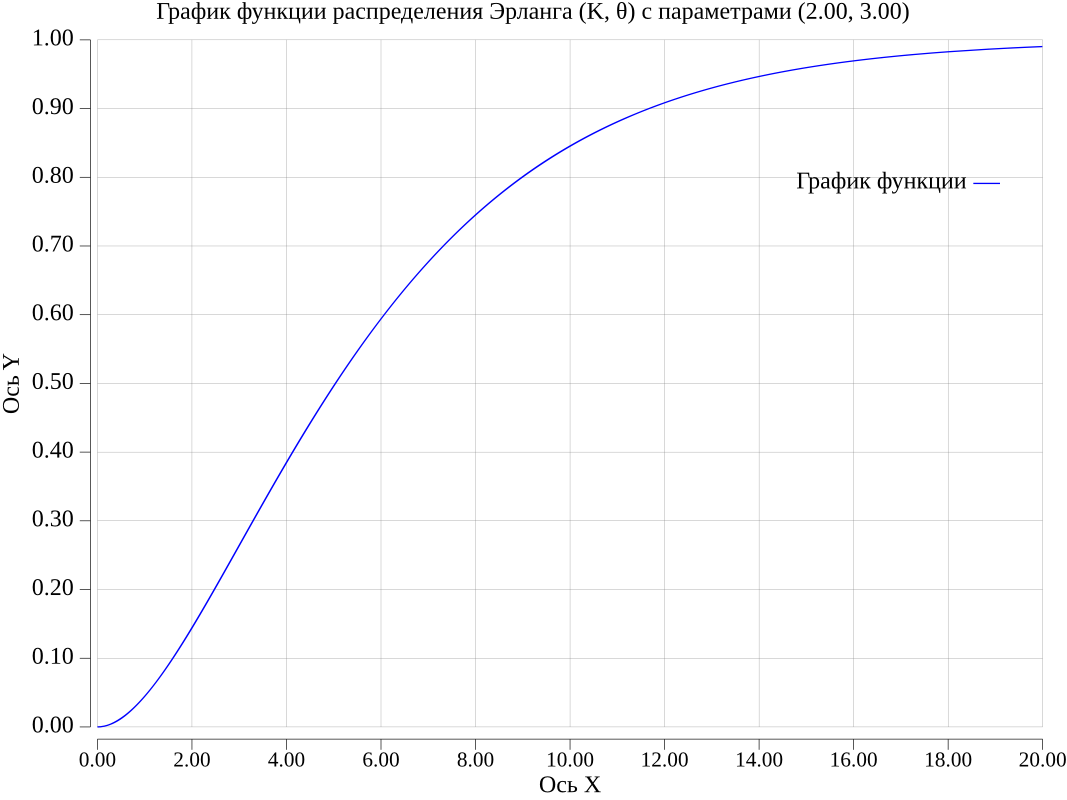
\includegraphics[width=\linewidth, height=12cm]{inc/erlangFunc.png}
	\end{center}
	\caption{Демонстрация построения графика функции распределения для распределения Эрланга}
\end{figure}
\FloatBarrier